\documentclass{standalone}

\begin{document}

% https://medium.com/the-theory-of-everything/understanding-activation-functions-in-neural-networks-9491262884e0
% https://towardsdatascience.com/activation-functions-and-its-types-which-is-better-a9a5310cc8f
% https://towardsdatascience.com/activation-functions-neural-networks-1cbd9f8d91d6

\section[Activation functions]{Activation Functions}\label{NN:activation}

Activation functions (or transfer functions) are linear or non linear equations which process the output of a Neural Network neuron and bound it into a limit range of values (commonly $\in[0, 1]$ or $\in[-1, 1]$).
The output of simple neuron\footnote{
  We assume for simplicity a fully connected Neural Network neuron.
} can be computed as dot product of the input and neuron weights (see previous section); in this case the output values ranging from $-inf$ to $+inf$ and moreover it is just a simple linear function.
Linear functions are very simple to trait but they are limited in their complexity and thus in their learning power.
Neural Networks without activation functions are just simple linear regression model (see the fully connected Neural Network properties in the previous section).
Neural Networks are considered as \emph{Universal Function Approximators} so the introduction of non-linearity allow them to model a wide range of functions and to learn more complex relations in the pattern data.
From a biological point of view the activation functions model the on/off state of a neuron in the output decision process.

Many activation functions were proposed during the years and each one has its characteristics but not an appropriate field of application.
The better activation function to use in a particular situation (to a particular problem) is still an open question.
Each one has its pro and cons in some situations so each Neural Network library implements a wide range of them and it leaves to the user to perform his own tests.
In Tab.~\ref{tab:activations} we show the list of activation functions implemented in our library with mathematical formulation and its derivative (ref. \href{https://github.com/Nico-Curti/NumPyNet/blob/master/NumPyNet/activations.py}{\textsf{activations.py}} for the code implementation).
An important feature of any activation function, in fact, is that it should be differentiable since the main procedure of model optimization implies the backpropagation of the error gradients.

\begin{table*}
\centering
\begin{adjustbox}{max width=\textwidth}
\begin{tabular}{lcc}
\hline \rowcolor{darkgrayrow}
\textbf{Name} & \textbf{Equation} & \textbf{Derivative} \\
\hline

Linear   &  $f(x) = x$                              &  $f'(x) = 1$ \\

Logistic &  $f(x) = \frac{1}{1 + \exp(-x)}$         &  $f'(x) = (1 - f(x)) * f(x)$ \\

Loggy    &  $f(x) = \frac{2}{1 + \exp(-x)} - 1$     &  $f'(x) = 2 * (1 - \frac{f(x) + 1}{2}) * \frac{f(x) + 1}{2} $ \\

Relu     &  $f(x) = \max(0, x)$                     &  $f'(x) = \left\{\begin{array}{rlr}
                                                                       1   & \mbox{if} & f(x) > 0    \\
                                                                       0   & \mbox{if} & f(x) \leq 0
                                                                       \end{array}\right.$           \\

Elu      &  $f(x) = \max(\exp(x) - 1, x)$           &  $f'(x) = \left\{\begin{array}{rlr}
                                                                       1        & \mbox{if} & f(x) \geq 0 \\
                                                                       f(x) + 1 & \mbox{if} & f(x) < 0
                                                                       \end{array}\right.$                \\

Relie    &  $f(x) = \max(x * 1e-2, x) $             &  $f'(x) = \left\{\begin{array}{rlr}
                                                                       1    & \mbox{if} & f(x) > 0    \\
                                                                       1e-2 & \mbox{if} & f(x) \leq 0
                                                                       \end{array}\right.$            \\

Ramp     &  $f(x) = \left\{\begin{array}{rlr}
                            x^2 + 0.1 * x^2 &  \mbox{if} & x > 0    \\
                            0               &  \mbox{if} & x \leq 0
                           \end{array}\right.$
                                                    &  $f'(x) = \left\{\begin{array}{rlr}
                                                                       f(x) + 1 & \mbox{if} & f(x) > 0   \\
                                                                       f(x)     & \mbox{if} & f(x) \leq 0
                                                                       \end{array}\right.$               \\

Tanh     &  $f(x) = \tanh(x)$                       &  $f'(x) = 1 - f(x)^2$  \\

Plse     &  $f(x) = \left\{\begin{array}{rlr}
                            (x + 4) * 1e-2     & \mbox{if} & x < -4           \\
                            (x - 4) * 1e-2 + 1 & \mbox{if} & x > 4            \\
                            x * 0.125 + 5      & \mbox{if} & -4 \leq x \leq 4
                           \end{array}\right.$
                                                    &  $f'(x) = \left\{\begin{array}{rlr}
                                                                       1e-2  & \mbox{if } & f(x) < 0 \mbox{ or } f(x) > 1 \\
                                                                       0.125 & \mbox{if } & 0 \leq f(x) \leq 1
                                                                       \end{array}\right.$                                \\

Leaky    &  $f(x) = \left\{\begin{array}{rlr}
                            x * C &  \mbox{if} & x \leq 0 \\
                            x     &  \mbox{if} & x > 0
                           \end{array}\right.$
                                                    &  $f'(x) = \left\{\begin{array}{rlr}
                                                                       1   & \mbox{if} & f(x) > 0    \\
                                                                       C   & \mbox{if} & f(x) \leq 0
                                                                       \end{array}\right.$           \\

HardTan  &  $f(x) = \left\{\begin{array}{rlr}
                            -1 & \mbox{if} &     x < -1 \\
                            +1 & \mbox{if} &     x > 1  \\
                             x & \mbox{if} & -1 \leq x \leq 1
                           \end{array}\right.$
                                                    &  $f'(x) = \left\{\begin{array}{rlr}
                                                                        0 & \mbox{if} & f(x) < -1 \mbox{ or } f(x) > 1 \\
                                                                        1 & \mbox{if} & -1 \leq f(x) \leq 1
                                                                       \end{array}\right.$                            \\

LhTan    &  $f(x) = \left\{\begin{array}{rlr}
                            x * 1e-3           & \mbox{if} &     x < 0  \\
                            (x - 1) * 1e-3 + 1 & \mbox{if} &     x > 1  \\
                             x                 & \mbox{if} & 0 \leq x \leq 1
                           \end{array}\right.$
                                                    &  $f'(x) = \left\{\begin{array}{rlr}
                                                                        1e-3           & \mbox{if} & f(x) < 0 \mbox{ or } f(x) > 1 \\
                                                                        1              & \mbox{if} & 0 \leq f(x) \leq 1
                                                                       \end{array}\right.$                                  \\

Selu     &  $f(x) =\left\{\begin{array}{rlr}
                            1.0507 * 1.6732 * (e^x - 1) & \mbox{if} &    x < 0  \\
                            x * 1.0507                  & \mbox{if} &    x \geq 0
                           \end{array}\right.$

                                                    &  $f'(x) = \left\{\begin{array}{rlr}
                                                                        f(x) * 1e-3           & \mbox{if} & f(x) 0    \\
                                                                        (f(x) - 1) * 1e-3 + 1 & \mbox{if} & f(x) > 1  \\
                                                                        \end{array}\right.$                           \\

SoftPlus &  $f(x) = log(1 + e^{x})$                 &  $f'(x) = \frac{\exp(f(x)}){1 + e^{f(x)}}$ \\

SoftSign &  $f(x) = \frac{x}{|x| + 1}$              &  $f'(x) = \frac{1}{(|f(x)| + 1)^{2}}$ \\

Elliot   &  $f(x) = \frac{\frac{1}{2} * S * x}{1 + |x + S|} + \frac{1}{2}$

                                                    &  $f'(x) = \frac{\frac{1}{2} * S}{(1 + |f(x) + S|)^{2}} $ \\

SymmElliot &  $f(x) = \frac{S * x}{1 + |x * S|}$    &  $f'(x) = \frac{S}{(1 + |f(x) * S|)^{2}}$ \\


%Swish    &  $f(x) = $                               &  $f'(x) = $                                                                                            %\\

%SoftMax  &  $f(x) =\frac{\exp(x)}{\sum_{i=1}^{N}x}$ &  $f'(x) = $


\hline\\
\end{tabular}
\end{adjustbox}
\caption{List of common activation functions with their correspondig mathematical equation and derivative.
The derivative is expressed as function of $f(x)$ to optimize their numerical evaluation.
}
\label{tab:activations}
\end{table*}

As can be seen in Tab.~\ref{tab:activations} it is easier to compute the activation function derivative as function of it.
This is a (well known) important type of optimization in computation term since it reduces the number of operations and it allows to apply the backward gradient directly.

%% move this paragraph to numpynet chapter!
To better understand the effects of activation functions we can perform these functions on a simple test image and comment the results.
This can be easy done using the example scripts inserted inside our library\footnote{
  Aware of the author no other example implementations have been done.
  This makes the NumPyNet library a useful tool for neural network study.
}.

\begin{center}
\begin{figure}[htbp]
\centering
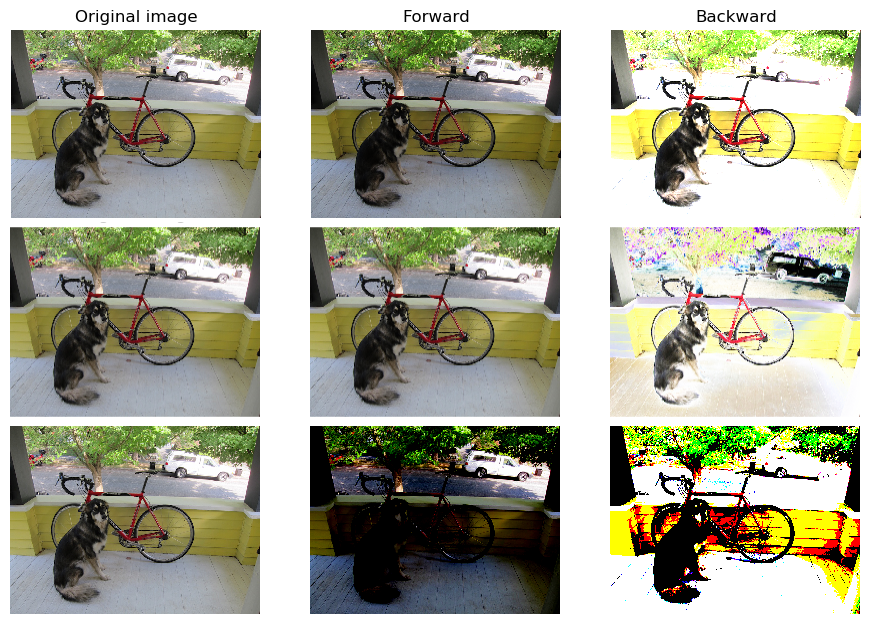
\includegraphics[width=0.85\textwidth]{activations_layer.png}
\caption{Activation functions applied on a testing image.
\textbf{(top)} Elu function and corresponding gradient.
\textbf{(center)} Logistic function and corresponding gradient.
\textbf{(bottom)} Relu function and corresponding gradient.
}
\label{fig:activations}
\end{figure}
\end{center}

In Fig.~\ref{fig:activations} the effects of the told above functions are reported on a test image.
For each function we show the output of the activation and its gradient.
For visualization purposes the image values are rescaled $\in[-1, 1]$ before the input to the functions.


% The question was which one is better to use ?
% Answer to this question is that nowadays we should use ReLu which should only be applied to the hidden layers. And if your model suffers form dead neurons during training we should use leaky ReLu or Maxout function.
% It’s just that Sigmoid and Tanh should not be used nowadays due to the vanishing Gradient Problem which causes a lots of problems to train,degrades the accuracy and performance of a deep Neural Network Model.


% Ok, now which one do we use?
% Now, which activation functions to use. Does that mean we just use ReLu for everything we do? Or sigmoid or tanh? Well, yes and no. When you know the function you are trying to approximate has certain characteristics, you can choose an activation function which will approximate the function faster leading to faster training process. For example, a sigmoid works well for a classifier ( see the graph of sigmoid, doesn’t it show the properties of an ideal classifier? ) because approximating a classifier function as combinations of sigmoid is easier than maybe ReLu, for example. Which will lead to faster training process and convergence. You can use your own custom functions too!. If you don’t know the nature of the function you are trying to learn, then maybe i would suggest start with ReLu, and then work backwards. ReLu works most of the time as a general approximator!
% In this article, I tried to describe a few activation functions used commonly. There are other activation functions too, but the general idea remains the same. Research for better activation functions is still ongoing. Hope you got the idea behind activation function, why they are used and how do we decide which one to use.


% CHOOSING THE RIGHT ACTIVATION FUNCTION
% The basic rule of thumb is if you really don’t know what activation function to use, then simply use RELU as it is a general activation function and is used in most cases these days.
% If your output is for binary classification then, sigmoid function is very natural choice for output layer.

\end{document}
